\section{Logical View}
Die logische Sicht beschreibt die Funktionalität der Komponenten.
Dazu wird ein UML-Klassendiagramm für jeden Microservice bereitgestellt.
Um die Lesbarkeit zu verbessern, werden die Bibliotheksklassen von \textit{Spring} und \textit{Fastify} nicht in den Diagrammen dargestellt.
Zusätzlich sind der Entity- sowie der Tracking-Service nicht in einem objektorientierten Stil mit TypeScript entwickelt worden.
Da sie keine Klassen verwenden, basieren ihre Klassendiagramme nicht auf Klassen, sondern auf deren Modulen.
Dadurch können die Funktionalitäten ähnlich zu einem klassischen Klassendiagramm abgebildet werden.

\subsection{Entity-Service}
\begin{figure}[!ht]
    \centering
    \makebox[0pt]{%
    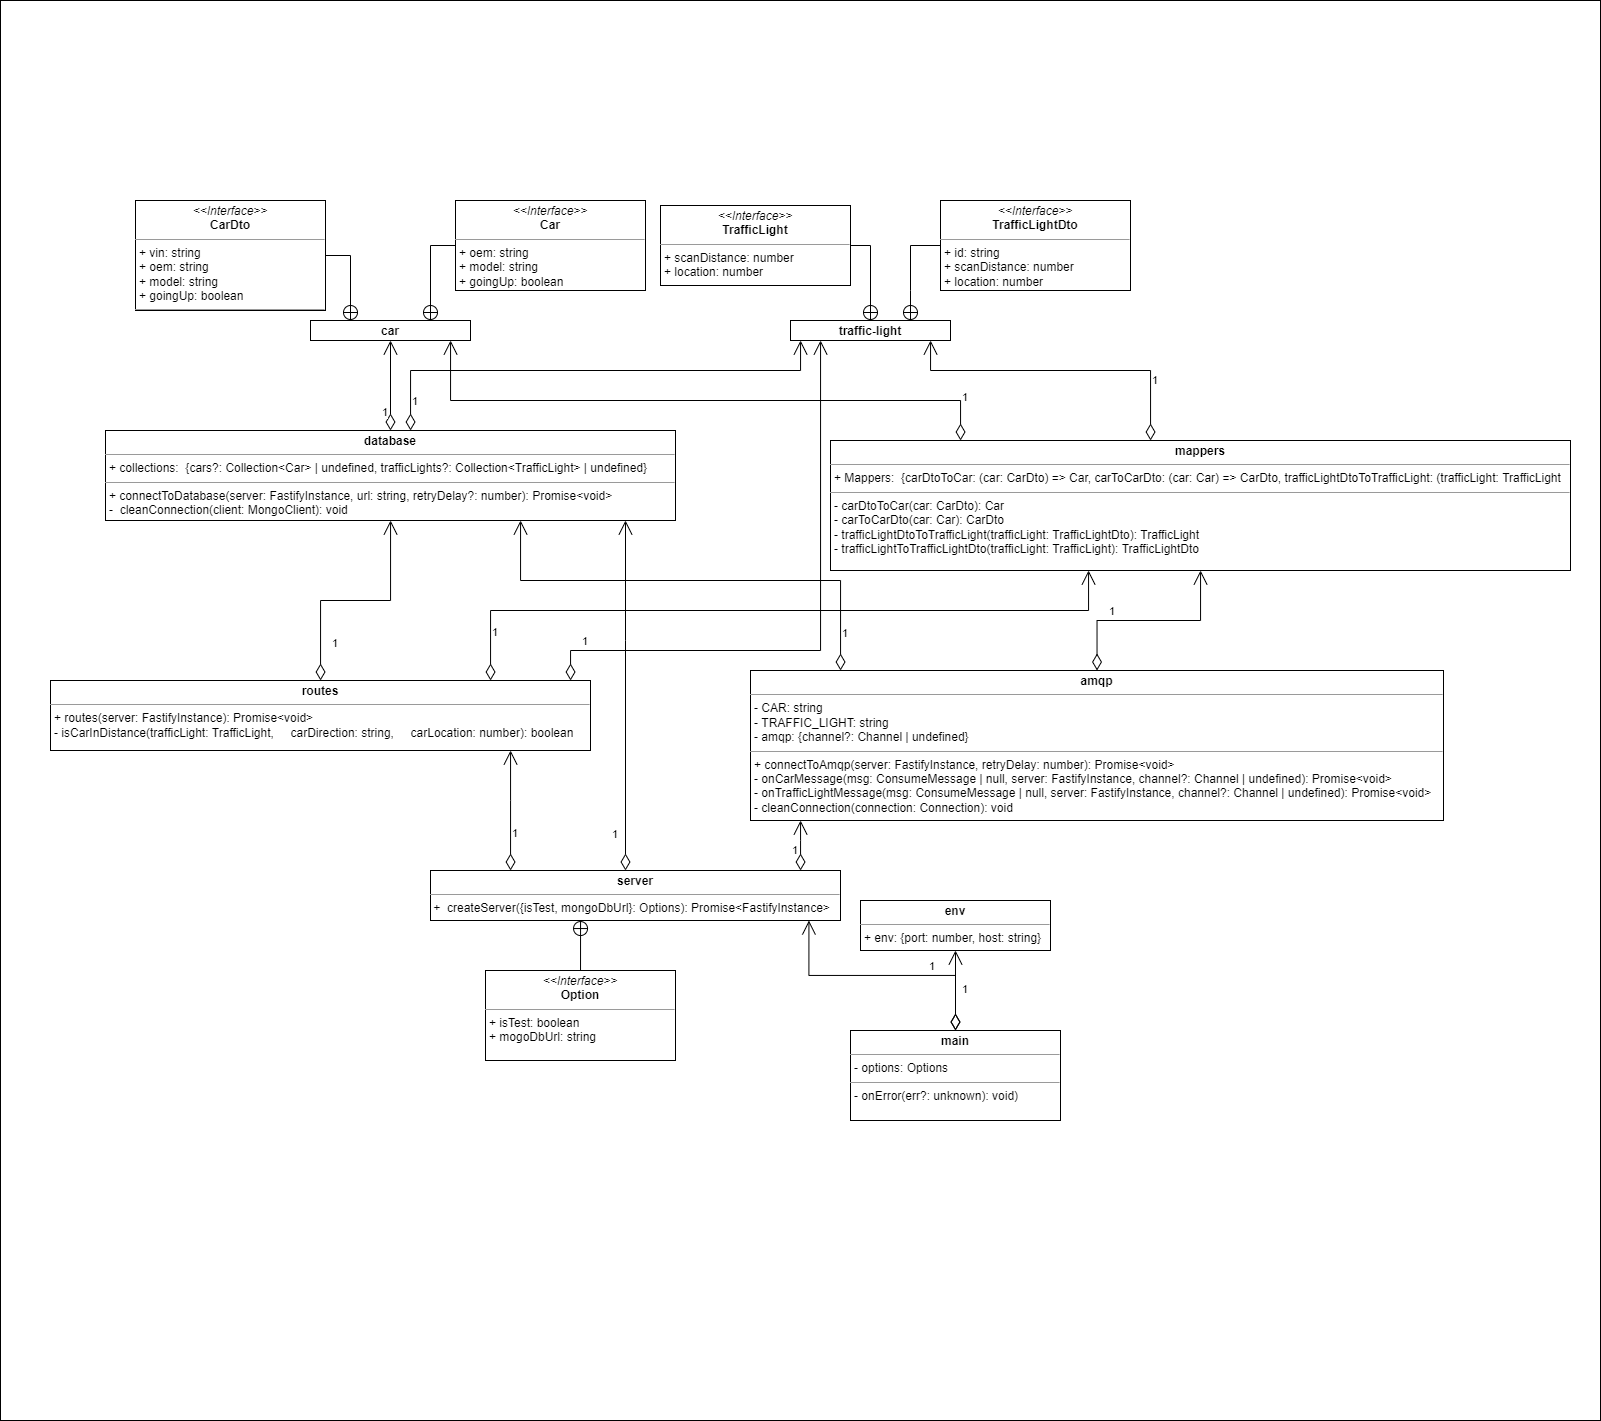
\includegraphics[width=18cm]{./figures/entity-service-uml.png}}
    \caption{Entity-Service UML}
    \label{fig:entity-service}
\end{figure}
\subsection{Tracking-Service}
\begin{figure}[!ht]
    \centering
    \makebox[0pt]{%
    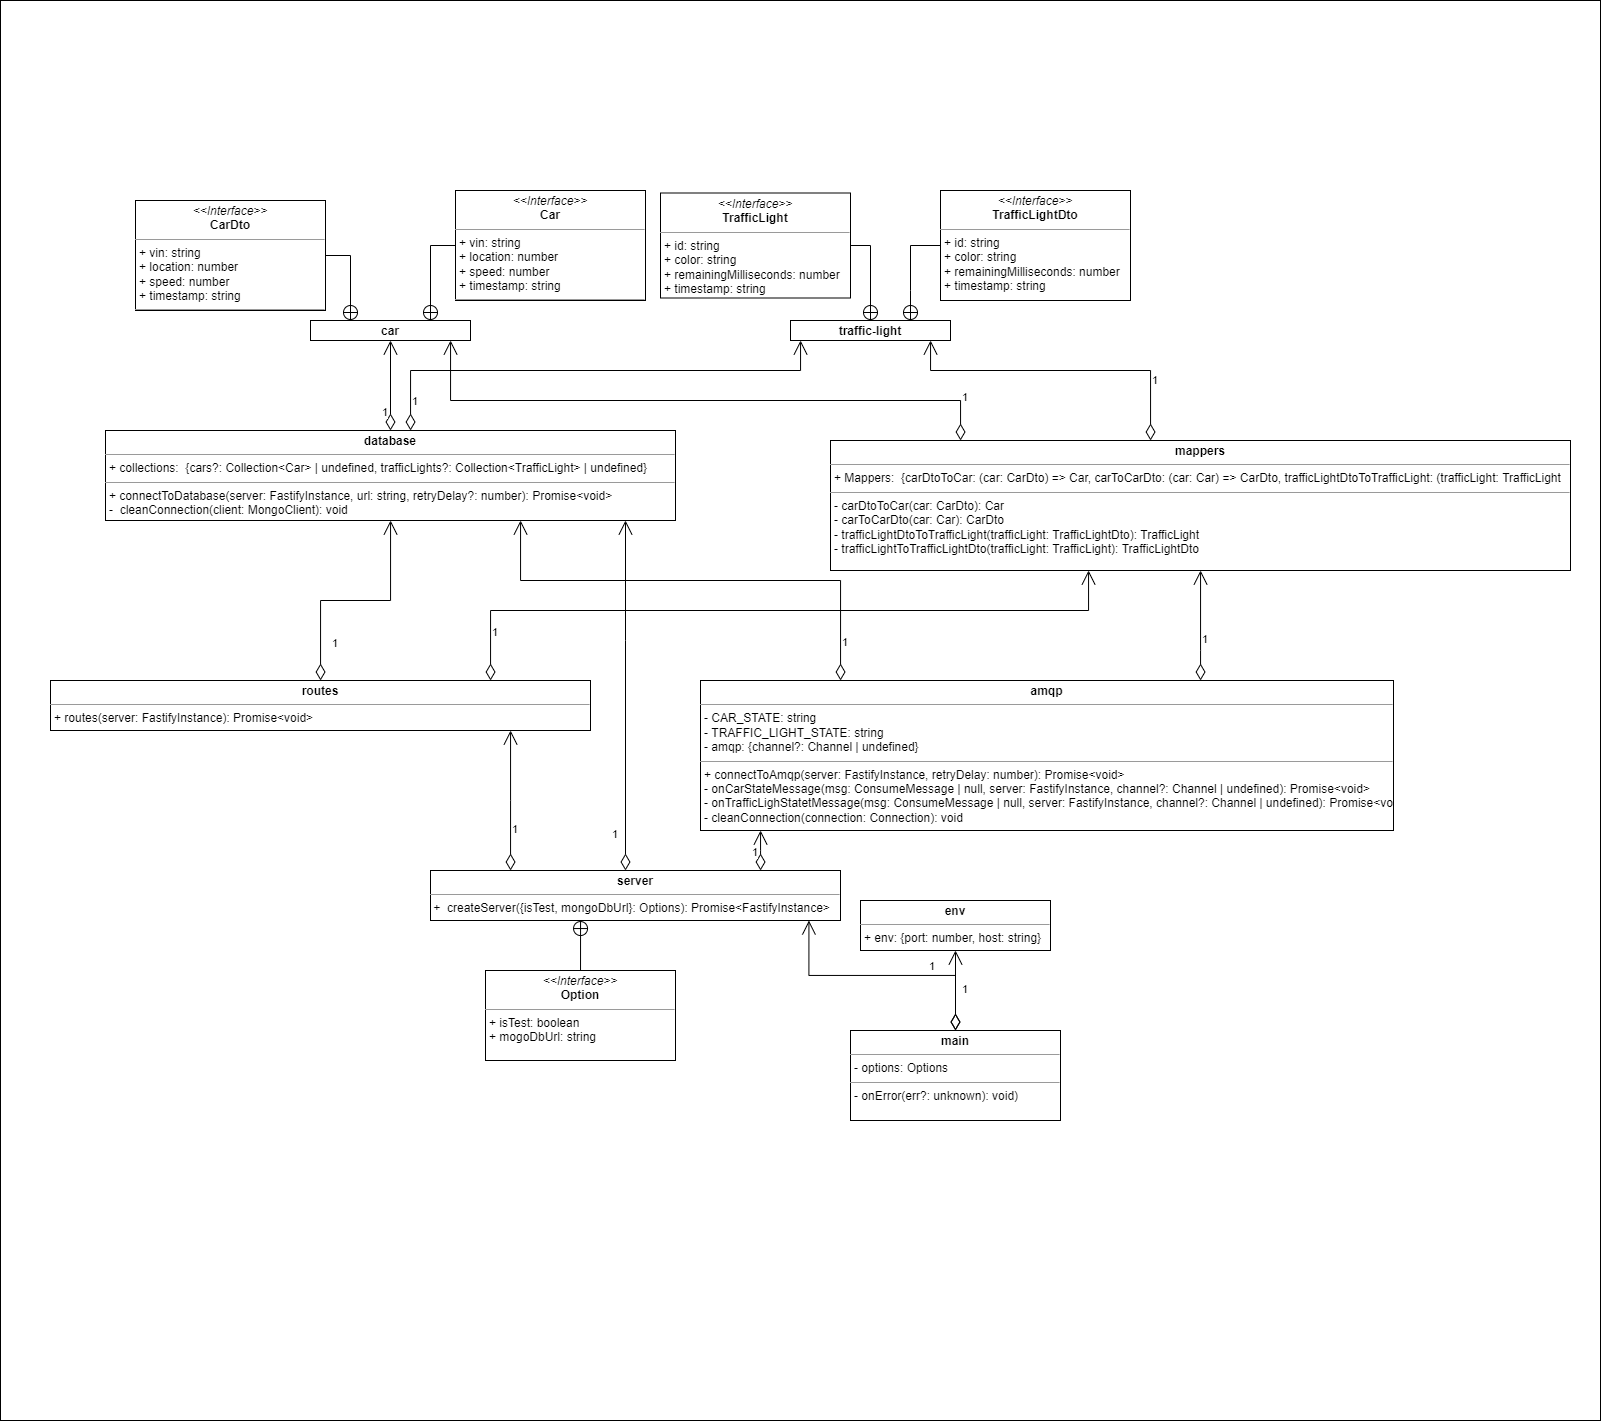
\includegraphics[width=18cm]{./figures/tracking-service.png}}
    \caption{Tracking-Service UML}
    \label{fig:tracking-service}
\end{figure}

\subsection{Gateway-Service}
\begin{figure}[!ht]
    \centering
    \makebox[0pt]{%
    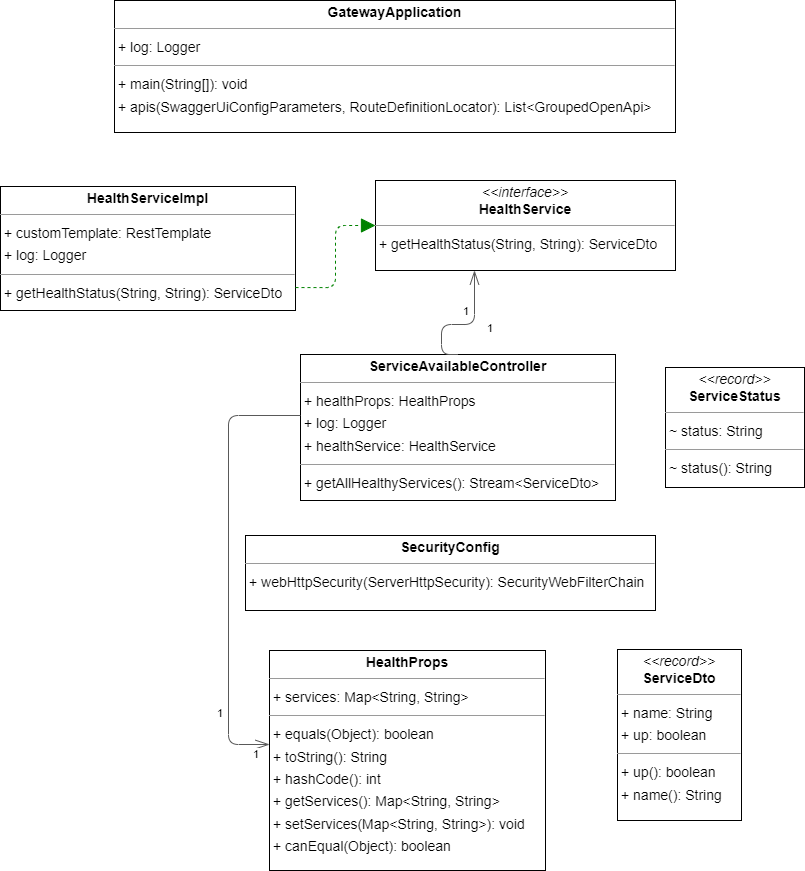
\includegraphics[width=18cm]{./figures/gateway-service.png}}
    \caption{Gateway-Service UML}
    \label{fig:gateway-service}
\end{figure}
\subsection{Simulator-Service}

\begin{figure}[!ht]
    \centering
    \makebox[0pt]{%
    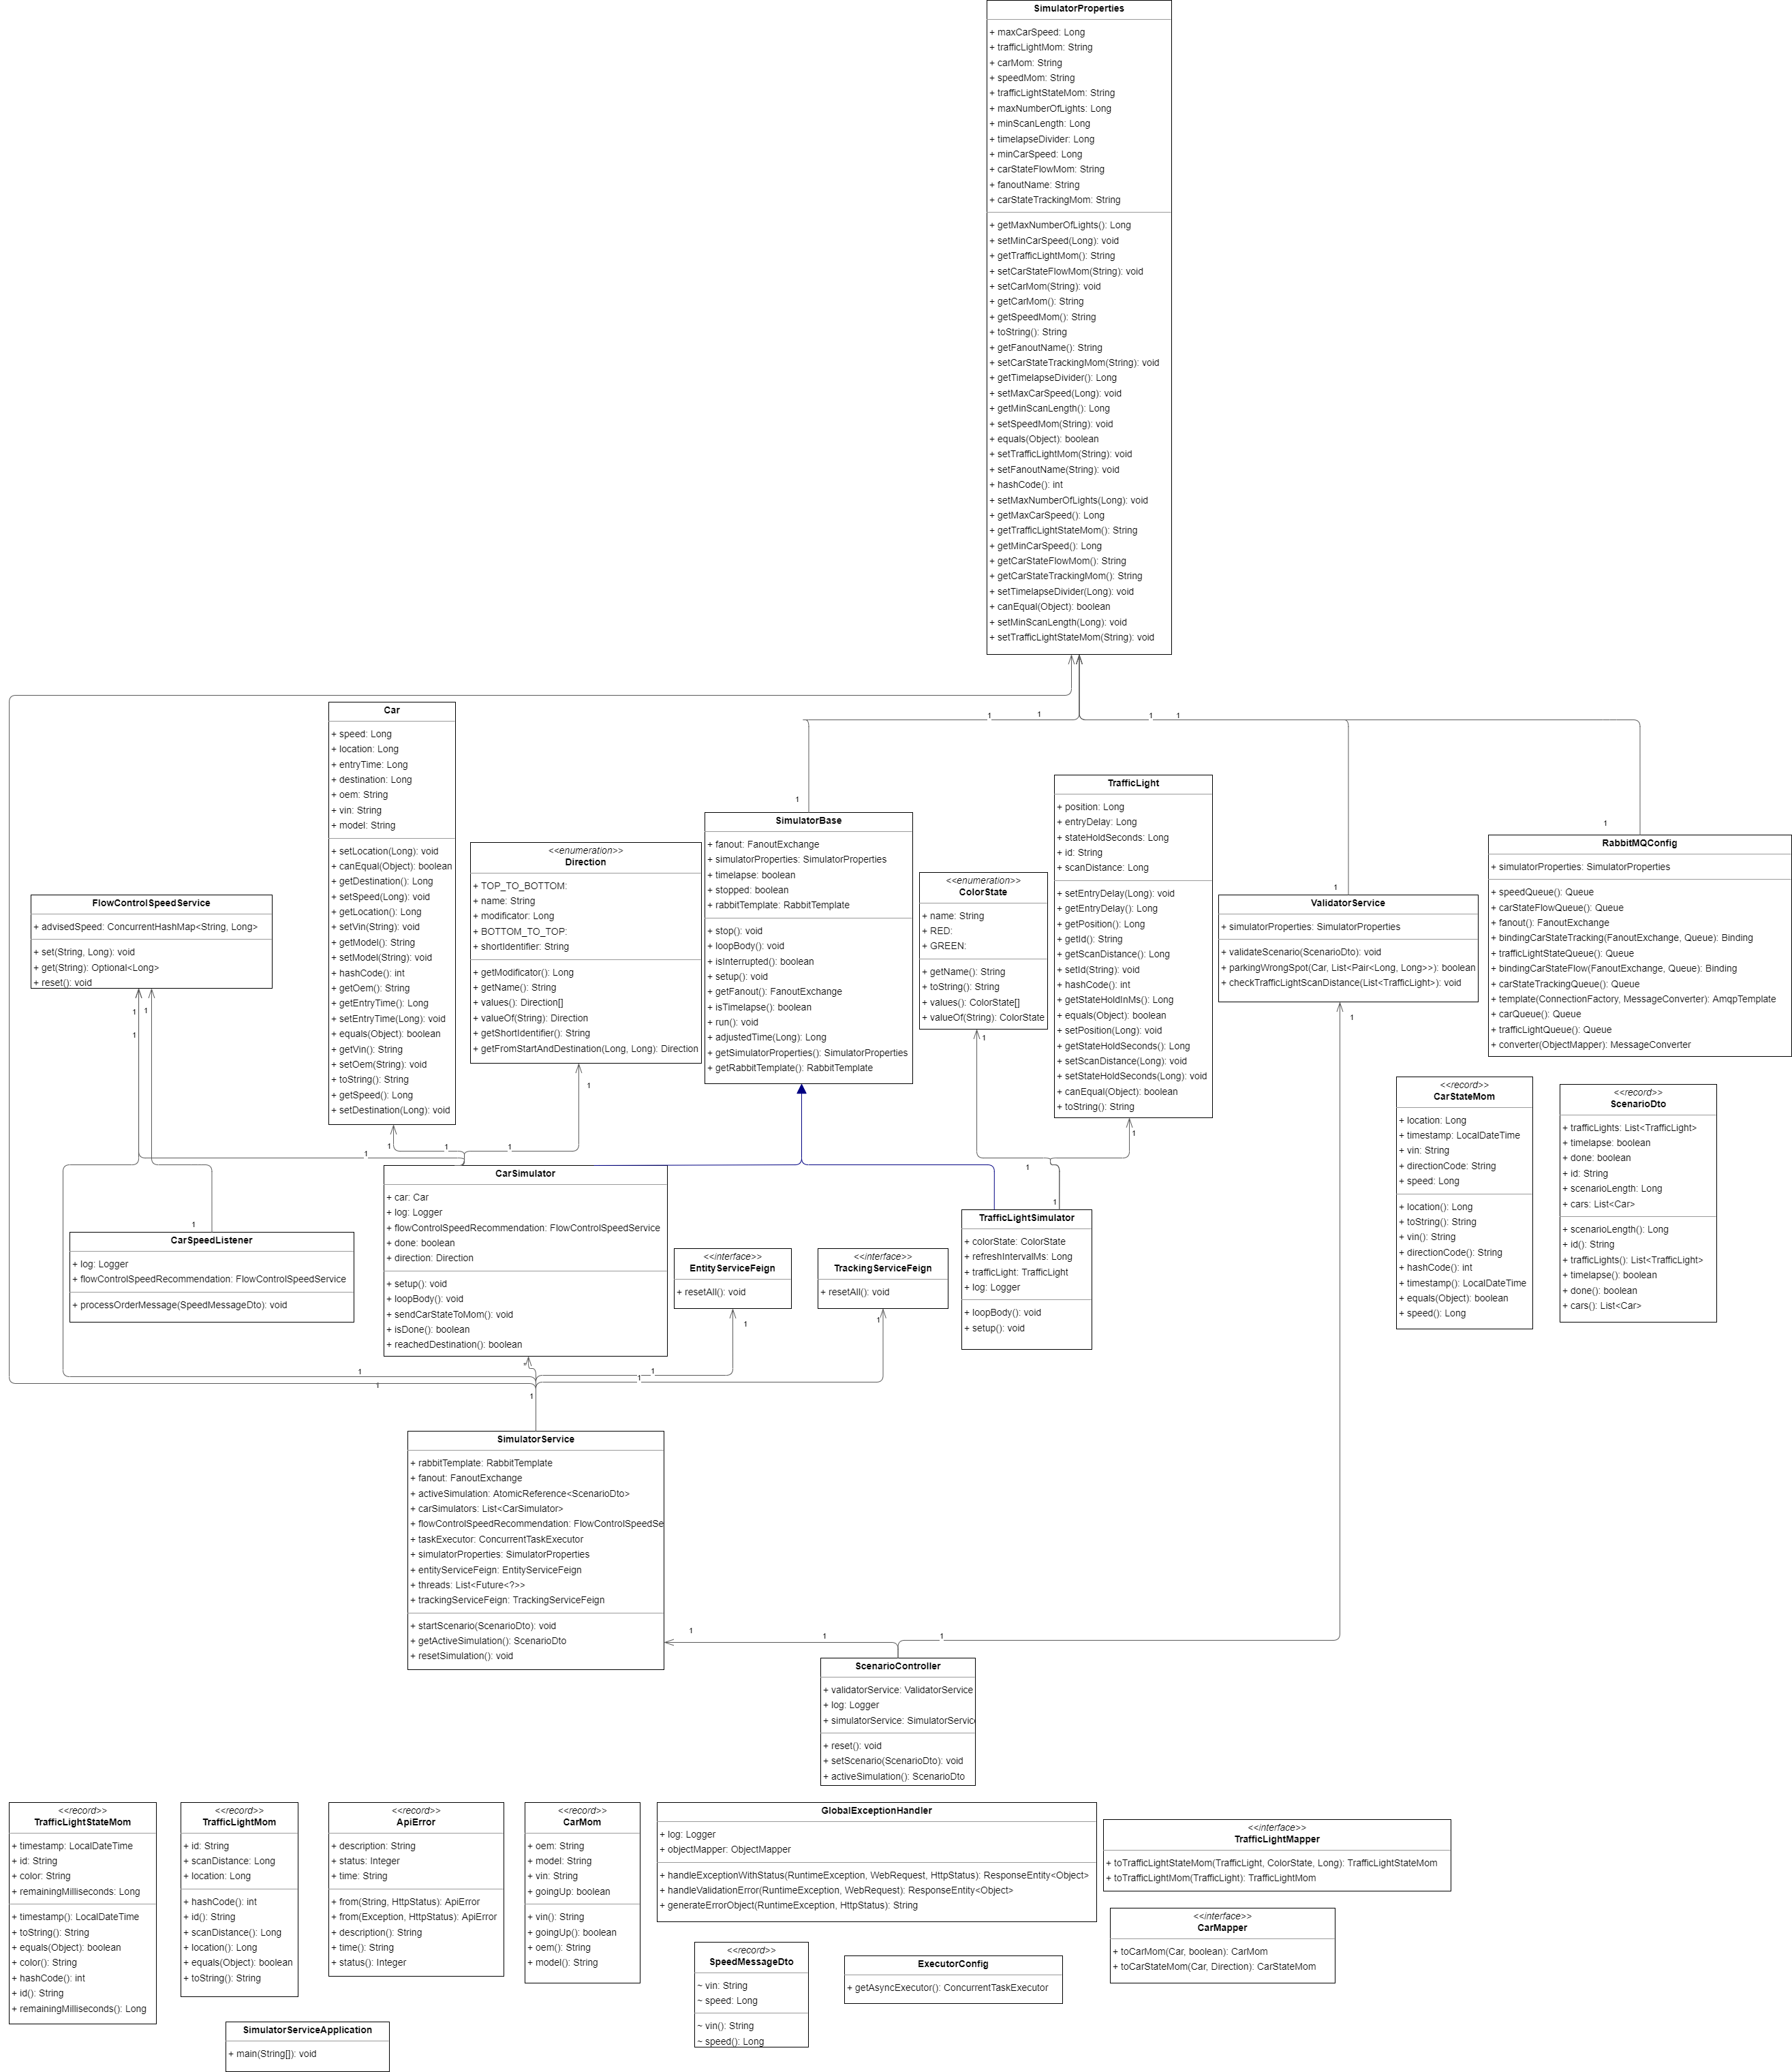
\includegraphics[width=18cm]{./figures/simulator-service.png}}
    \caption{Simulator-Service UML}
    \label{fig:simulator-service}
\end{figure}

\subsection{Flowcontrol-Service}

\begin{figure}[!ht]
    \centering
    \makebox[0pt]{%
    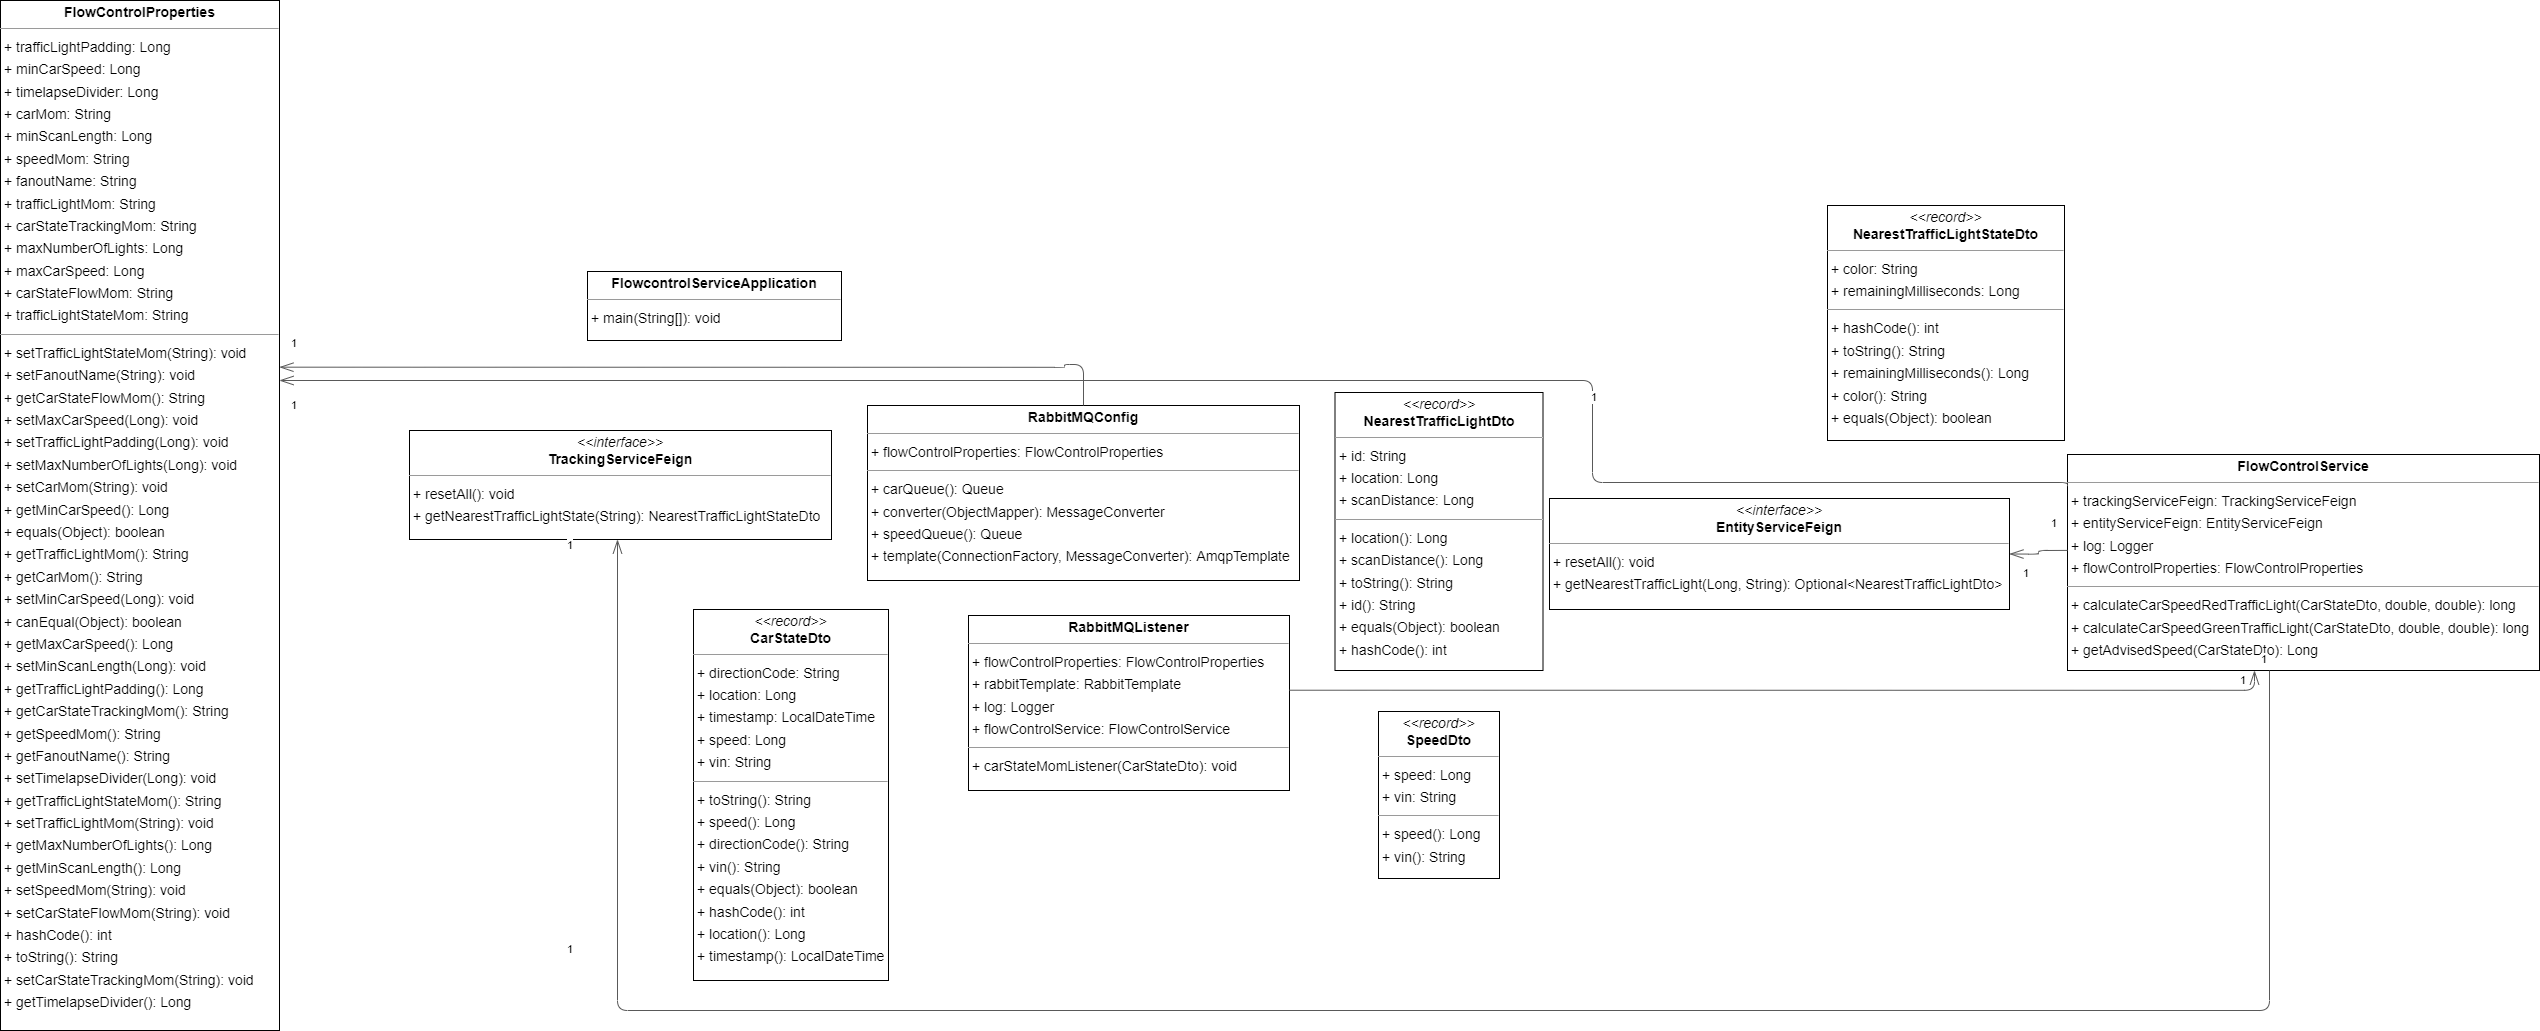
\includegraphics[width=18cm]{./figures/flowcontrol.png}}
    \caption{Flowcontrol-Service UML}
    \label{fig:flowcontrol-service}
\end{figure}
